\chapter{Исследовательская часть}

В данном разделе будет описано тестирование реализованного анализатора изображений.

\section{Образец отчёта без ошибок}
На рисунке \ref{img:pos} представлен скриншот электронного отчёта, не содержащий нарушений интервала после и до заголовка раздела (подраздела).

\begin{figure}
	\centering
	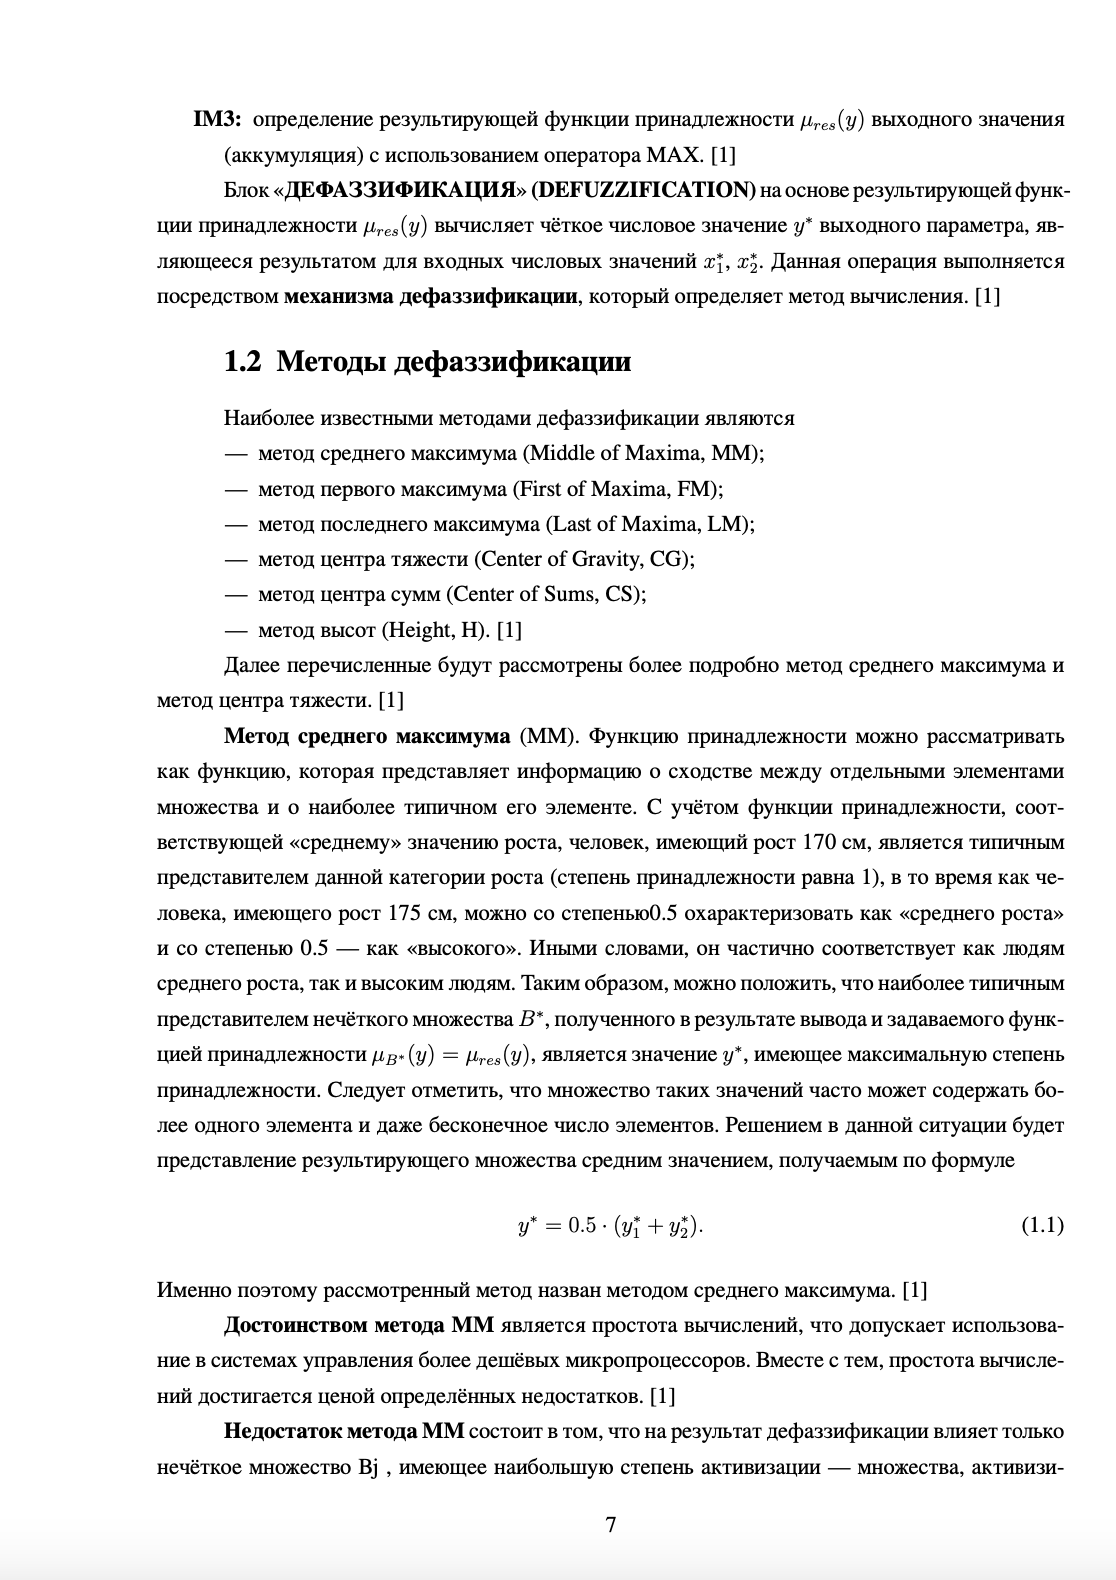
\includegraphics[width=0.9\textwidth]{images/pos.png}
	\caption{Образец отчёта без ошибок}
	\label{img:pos}
\end{figure}

Реализованный анализатор не выявил нарушений.

\section{Образец отчёта без ошибок}
На рисунках \ref{img:neg1} и \ref{img:neg2} представлены скриншоты электронных отчётов, содержащие нарушения интервала после и до заголовка раздела (подраздела).

\begin{figure}
	\centering
	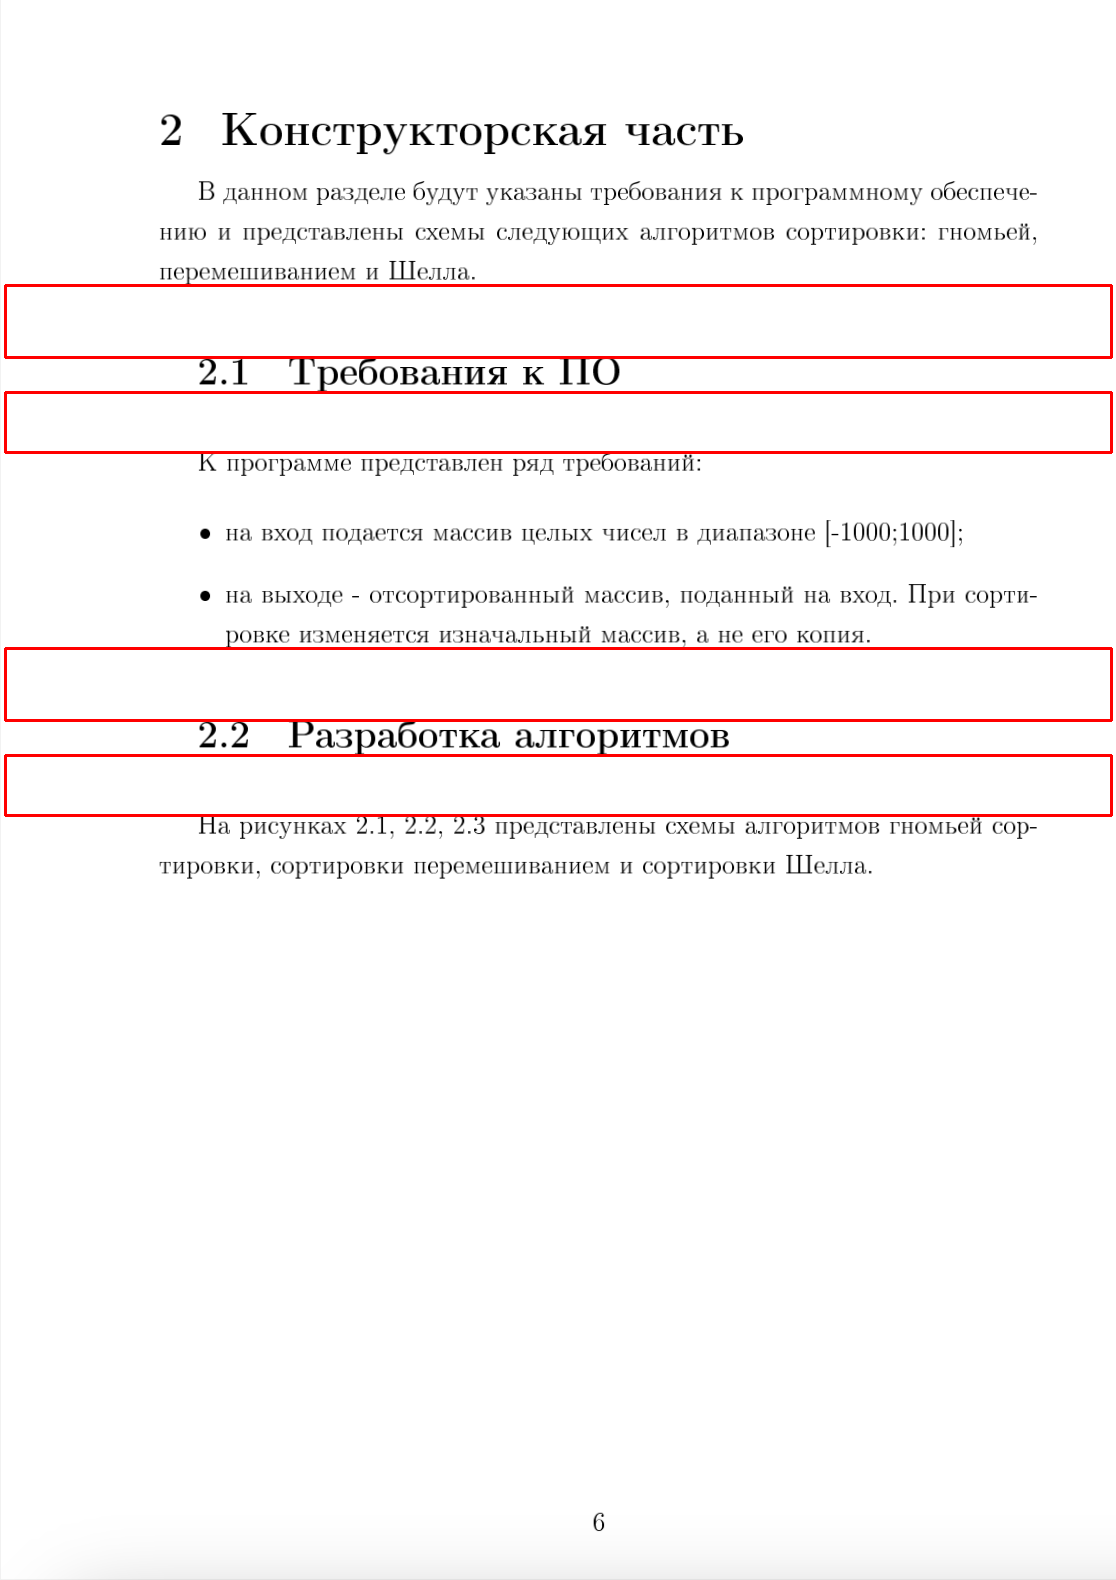
\includegraphics[width=0.9\textwidth]{images/neg1.png}
	\caption{Образец отчёта с ошибками (1)}
	\label{img:neg1}
\end{figure}

\begin{figure}
	\centering
	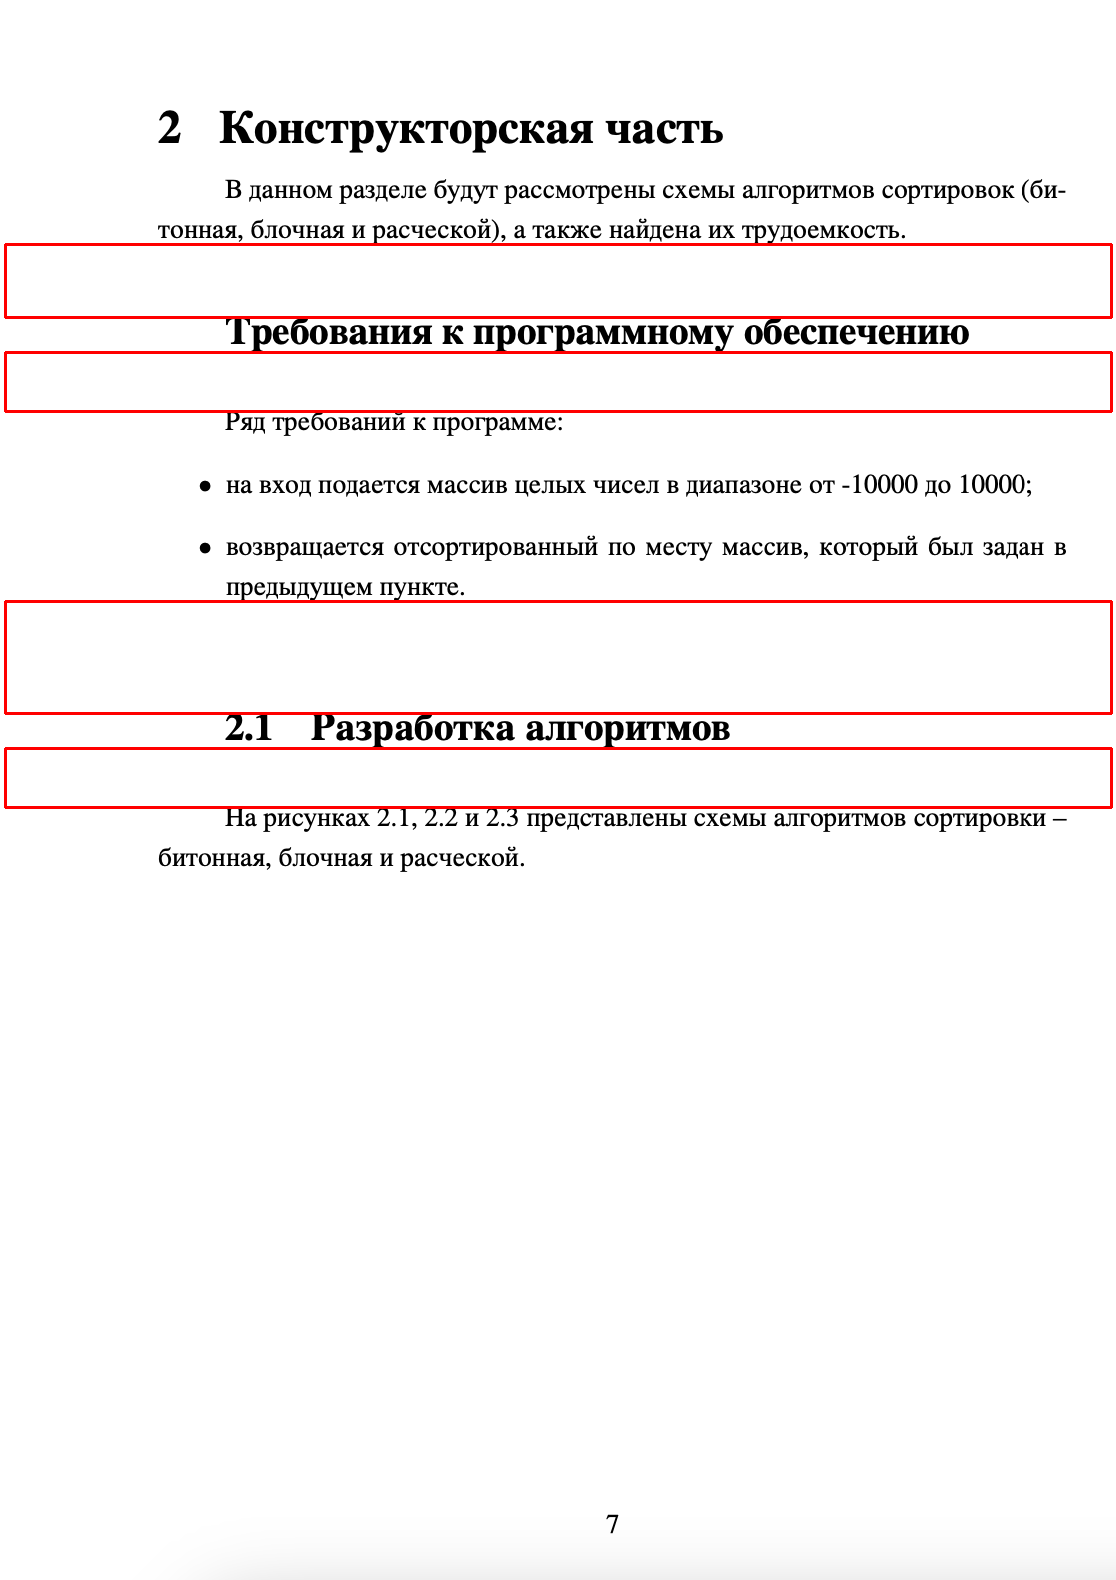
\includegraphics[width=0.9\textwidth]{images/neg2.png}
	\caption{Образец отчёта с ошибками (2)}
	\label{img:neg2}
\end{figure}

Выявленные нарушения анализатор выделил красным цветом.

\section*{Вывод}

Реализованный анализатор успешно прошёл тесты на реальных отчётах студентов. Тот факт, что в коде программы не используются абсолютные величины (высоты текста, отступов и т.д.), позволяет не предъявлять требований к разрешению анализируемых изображений.

\clearpage
